\begin{figure}[H] \centering % Created by tikzDevice version 0.12.4 on 2023-07-23 21:18:17
% !TEX encoding = UTF-8 Unicode
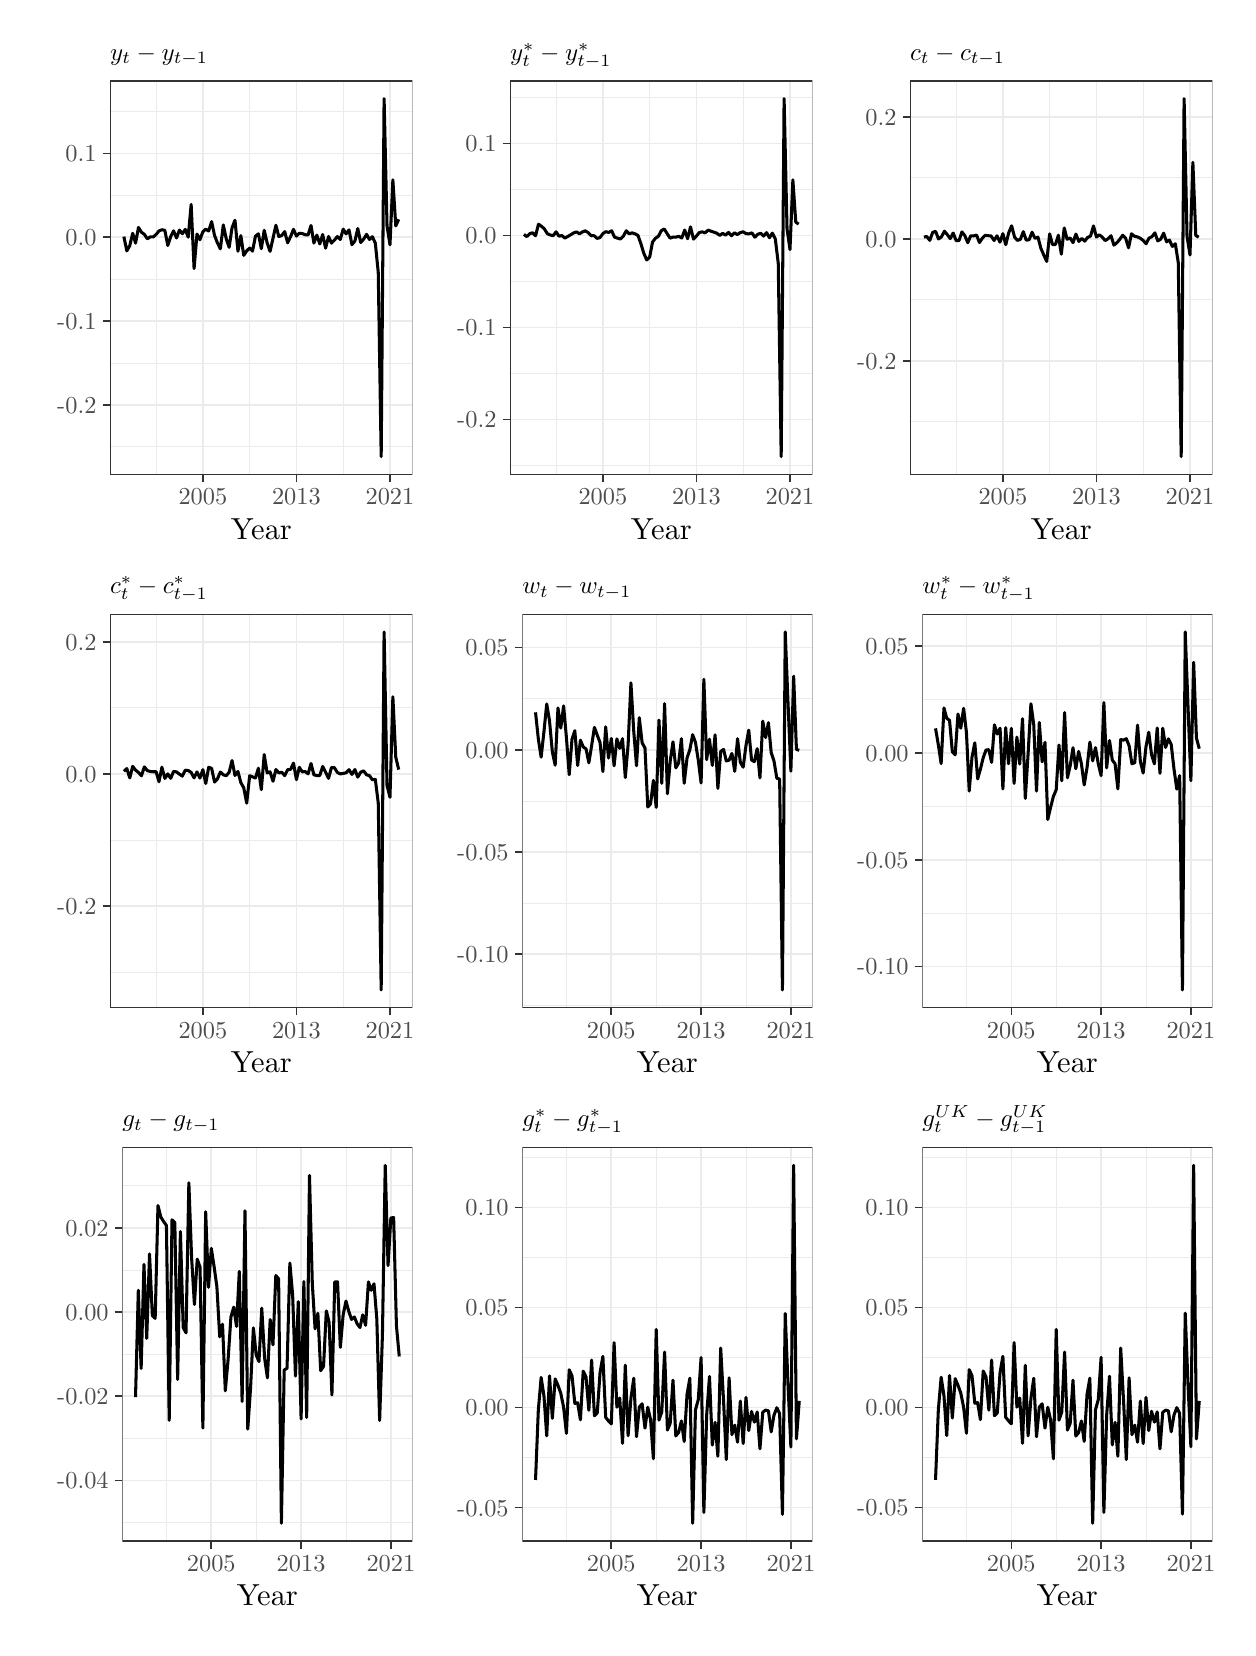
\begin{tikzpicture}[x=1pt,y=1pt]
\definecolor{fillColor}{RGB}{255,255,255}
\path[use as bounding box,fill=fillColor,fill opacity=0.00] (0,0) rectangle (433.62,578.16);
\begin{scope}
\path[clip] (  0.00,385.44) rectangle (144.54,578.16);
\definecolor{drawColor}{RGB}{255,255,255}
\definecolor{fillColor}{RGB}{255,255,255}

\path[draw=drawColor,line width= 0.6pt,line join=round,line cap=round,fill=fillColor] ( -0.00,385.44) rectangle (144.54,578.16);
\end{scope}
\begin{scope}
\path[clip] ( 29.80,416.69) rectangle (139.04,558.97);
\definecolor{fillColor}{RGB}{255,255,255}

\path[fill=fillColor] ( 29.80,416.69) rectangle (139.04,558.97);
\definecolor{drawColor}{gray}{0.92}

\path[draw=drawColor,line width= 0.3pt,line join=round] ( 29.80,426.73) --
	(139.04,426.73);

\path[draw=drawColor,line width= 0.3pt,line join=round] ( 29.80,457.00) --
	(139.04,457.00);

\path[draw=drawColor,line width= 0.3pt,line join=round] ( 29.80,487.26) --
	(139.04,487.26);

\path[draw=drawColor,line width= 0.3pt,line join=round] ( 29.80,517.53) --
	(139.04,517.53);

\path[draw=drawColor,line width= 0.3pt,line join=round] ( 29.80,547.79) --
	(139.04,547.79);

\path[draw=drawColor,line width= 0.3pt,line join=round] ( 46.41,416.69) --
	( 46.41,558.97);

\path[draw=drawColor,line width= 0.3pt,line join=round] ( 80.21,416.69) --
	( 80.21,558.97);

\path[draw=drawColor,line width= 0.3pt,line join=round] (114.01,416.69) --
	(114.01,558.97);

\path[draw=drawColor,line width= 0.6pt,line join=round] ( 29.80,441.87) --
	(139.04,441.87);

\path[draw=drawColor,line width= 0.6pt,line join=round] ( 29.80,472.13) --
	(139.04,472.13);

\path[draw=drawColor,line width= 0.6pt,line join=round] ( 29.80,502.40) --
	(139.04,502.40);

\path[draw=drawColor,line width= 0.6pt,line join=round] ( 29.80,532.66) --
	(139.04,532.66);

\path[draw=drawColor,line width= 0.6pt,line join=round] ( 63.31,416.69) --
	( 63.31,558.97);

\path[draw=drawColor,line width= 0.6pt,line join=round] ( 97.11,416.69) --
	( 97.11,558.97);

\path[draw=drawColor,line width= 0.6pt,line join=round] (130.92,416.69) --
	(130.92,558.97);
\definecolor{drawColor}{RGB}{0,0,0}

\path[draw=drawColor,line width= 1.1pt,line join=round] ( 34.77,502.66) --
	( 35.82,497.48) --
	( 36.89,499.38) --
	( 37.95,503.86) --
	( 38.99,500.29) --
	( 40.04,505.95) --
	( 41.11,504.24) --
	( 42.17,503.44) --
	( 43.23,501.86) --
	( 44.28,502.54) --
	( 45.34,502.52) --
	( 46.41,503.42) --
	( 47.45,504.71) --
	( 48.50,505.14) --
	( 49.57,504.92) --
	( 50.63,499.44) --
	( 51.67,502.61) --
	( 52.72,504.74) --
	( 53.79,502.15) --
	( 54.85,505.03) --
	( 55.89,503.69) --
	( 56.95,505.26) --
	( 58.01,502.46) --
	( 59.07,514.28) --
	( 60.13,491.11) --
	( 61.18,503.58) --
	( 62.24,501.52) --
	( 63.31,504.41) --
	( 64.35,505.36) --
	( 65.40,504.66) --
	( 66.47,508.09) --
	( 67.53,503.06) --
	( 68.57,500.36) --
	( 69.63,498.23) --
	( 70.69,506.86) --
	( 71.75,501.89) --
	( 72.80,498.78) --
	( 73.85,505.86) --
	( 74.91,508.58) --
	( 75.98,497.36) --
	( 77.03,503.00) --
	( 78.08,495.89) --
	( 79.15,497.49) --
	( 80.21,498.53) --
	( 81.25,497.40) --
	( 82.30,502.78) --
	( 83.37,503.67) --
	( 84.43,498.28) --
	( 85.47,504.95) --
	( 86.53,500.38) --
	( 87.59,497.31) --
	( 88.66,502.11) --
	( 89.70,506.76) --
	( 90.75,502.66) --
	( 91.81,503.07) --
	( 92.88,504.47) --
	( 93.93,500.41) --
	( 94.98,502.61) --
	( 96.05,505.29) --
	( 97.11,502.85) --
	( 98.15,503.87) --
	( 99.21,503.77) --
	(100.27,503.34) --
	(101.34,503.27) --
	(102.38,506.68) --
	(103.43,500.33) --
	(104.49,503.19) --
	(105.56,500.00) --
	(106.60,503.40) --
	(107.65,498.46) --
	(108.72,502.71) --
	(109.78,500.30) --
	(110.83,501.38) --
	(111.89,502.67) --
	(112.95,501.61) --
	(114.01,505.36) --
	(115.06,503.65) --
	(116.11,505.07) --
	(117.17,499.75) --
	(118.24,501.04) --
	(119.28,505.58) --
	(120.33,500.51) --
	(121.40,501.74) --
	(122.46,503.48) --
	(123.50,501.62) --
	(124.55,502.62) --
	(125.62,500.29) --
	(126.68,489.70) --
	(127.74,423.16) --
	(128.79,552.51) --
	(129.85,506.49) --
	(130.92,499.70) --
	(131.96,523.16) --
	(133.01,506.52) --
	(134.07,508.90);
\definecolor{drawColor}{gray}{0.20}

\path[draw=drawColor,line width= 0.6pt,line join=round,line cap=round] ( 29.80,416.69) rectangle (139.04,558.97);
\end{scope}
\begin{scope}
\path[clip] (  0.00,  0.00) rectangle (433.62,578.16);
\definecolor{drawColor}{gray}{0.30}

\node[text=drawColor,anchor=base east,inner sep=0pt, outer sep=0pt, scale=  0.88] at ( 24.85,438.84) {-0.2};

\node[text=drawColor,anchor=base east,inner sep=0pt, outer sep=0pt, scale=  0.88] at ( 24.85,469.10) {-0.1};

\node[text=drawColor,anchor=base east,inner sep=0pt, outer sep=0pt, scale=  0.88] at ( 24.85,499.36) {0.0};

\node[text=drawColor,anchor=base east,inner sep=0pt, outer sep=0pt, scale=  0.88] at ( 24.85,529.63) {0.1};
\end{scope}
\begin{scope}
\path[clip] (  0.00,  0.00) rectangle (433.62,578.16);
\definecolor{drawColor}{gray}{0.20}

\path[draw=drawColor,line width= 0.6pt,line join=round] ( 27.05,441.87) --
	( 29.80,441.87);

\path[draw=drawColor,line width= 0.6pt,line join=round] ( 27.05,472.13) --
	( 29.80,472.13);

\path[draw=drawColor,line width= 0.6pt,line join=round] ( 27.05,502.40) --
	( 29.80,502.40);

\path[draw=drawColor,line width= 0.6pt,line join=round] ( 27.05,532.66) --
	( 29.80,532.66);
\end{scope}
\begin{scope}
\path[clip] (  0.00,  0.00) rectangle (433.62,578.16);
\definecolor{drawColor}{gray}{0.20}

\path[draw=drawColor,line width= 0.6pt,line join=round] ( 63.31,413.94) --
	( 63.31,416.69);

\path[draw=drawColor,line width= 0.6pt,line join=round] ( 97.11,413.94) --
	( 97.11,416.69);

\path[draw=drawColor,line width= 0.6pt,line join=round] (130.92,413.94) --
	(130.92,416.69);
\end{scope}
\begin{scope}
\path[clip] (  0.00,  0.00) rectangle (433.62,578.16);
\definecolor{drawColor}{gray}{0.30}

\node[text=drawColor,anchor=base,inner sep=0pt, outer sep=0pt, scale=  0.88] at ( 63.31,405.68) {2005};

\node[text=drawColor,anchor=base,inner sep=0pt, outer sep=0pt, scale=  0.88] at ( 97.11,405.68) {2013};

\node[text=drawColor,anchor=base,inner sep=0pt, outer sep=0pt, scale=  0.88] at (130.92,405.68) {2021};
\end{scope}
\begin{scope}
\path[clip] (  0.00,  0.00) rectangle (433.62,578.16);
\definecolor{drawColor}{RGB}{0,0,0}

\node[text=drawColor,anchor=base,inner sep=0pt, outer sep=0pt, scale=  1.10] at ( 84.42,393.37) {Year};
\end{scope}
\begin{scope}
\path[clip] (  0.00,  0.00) rectangle (433.62,578.16);
\definecolor{drawColor}{RGB}{0,0,0}

\node[text=drawColor,anchor=base west,inner sep=0pt, outer sep=0pt, scale=  0.90] at ( 29.80,566.46) {$y_t - y_{t-1}$};
\end{scope}
\begin{scope}
\path[clip] (144.54,385.44) rectangle (289.08,578.16);
\definecolor{drawColor}{RGB}{255,255,255}
\definecolor{fillColor}{RGB}{255,255,255}

\path[draw=drawColor,line width= 0.6pt,line join=round,line cap=round,fill=fillColor] (144.54,385.44) rectangle (289.08,578.16);
\end{scope}
\begin{scope}
\path[clip] (174.34,416.69) rectangle (283.58,558.97);
\definecolor{fillColor}{RGB}{255,255,255}

\path[fill=fillColor] (174.34,416.69) rectangle (283.58,558.97);
\definecolor{drawColor}{gray}{0.92}

\path[draw=drawColor,line width= 0.3pt,line join=round] (174.34,419.98) --
	(283.58,419.98);

\path[draw=drawColor,line width= 0.3pt,line join=round] (174.34,453.21) --
	(283.58,453.21);

\path[draw=drawColor,line width= 0.3pt,line join=round] (174.34,486.44) --
	(283.58,486.44);

\path[draw=drawColor,line width= 0.3pt,line join=round] (174.34,519.67) --
	(283.58,519.67);

\path[draw=drawColor,line width= 0.3pt,line join=round] (174.34,552.90) --
	(283.58,552.90);

\path[draw=drawColor,line width= 0.3pt,line join=round] (190.95,416.69) --
	(190.95,558.97);

\path[draw=drawColor,line width= 0.3pt,line join=round] (224.75,416.69) --
	(224.75,558.97);

\path[draw=drawColor,line width= 0.3pt,line join=round] (258.55,416.69) --
	(258.55,558.97);

\path[draw=drawColor,line width= 0.6pt,line join=round] (174.34,436.60) --
	(283.58,436.60);

\path[draw=drawColor,line width= 0.6pt,line join=round] (174.34,469.83) --
	(283.58,469.83);

\path[draw=drawColor,line width= 0.6pt,line join=round] (174.34,503.05) --
	(283.58,503.05);

\path[draw=drawColor,line width= 0.6pt,line join=round] (174.34,536.28) --
	(283.58,536.28);

\path[draw=drawColor,line width= 0.6pt,line join=round] (207.85,416.69) --
	(207.85,558.97);

\path[draw=drawColor,line width= 0.6pt,line join=round] (241.65,416.69) --
	(241.65,558.97);

\path[draw=drawColor,line width= 0.6pt,line join=round] (275.46,416.69) --
	(275.46,558.97);
\definecolor{drawColor}{RGB}{0,0,0}

\path[draw=drawColor,line width= 1.1pt,line join=round] (179.31,503.43) --
	(180.36,502.66) --
	(181.43,503.73) --
	(182.49,504.04) --
	(183.53,502.95) --
	(184.58,507.15) --
	(185.65,506.39) --
	(186.71,505.45) --
	(187.77,503.72) --
	(188.82,503.25) --
	(189.88,502.98) --
	(190.95,504.39) --
	(191.99,502.77) --
	(193.04,503.08) --
	(194.11,502.10) --
	(195.17,502.71) --
	(196.21,503.32) --
	(197.26,503.98) --
	(198.33,504.35) --
	(199.39,503.68) --
	(200.43,504.32) --
	(201.49,504.75) --
	(202.55,504.07) --
	(203.61,502.97) --
	(204.67,502.98) --
	(205.72,502.02) --
	(206.78,502.28) --
	(207.85,503.72) --
	(208.89,504.44) --
	(209.94,504.15) --
	(211.01,504.76) --
	(212.07,502.46) --
	(213.11,502.10) --
	(214.17,501.80) --
	(215.23,502.77) --
	(216.29,504.77) --
	(217.34,503.67) --
	(218.39,504.01) --
	(219.45,503.68) --
	(220.52,503.10) --
	(221.57,500.14) --
	(222.62,496.66) --
	(223.69,494.21) --
	(224.75,495.22) --
	(225.79,500.68) --
	(226.84,502.07) --
	(227.91,502.77) --
	(228.97,504.78) --
	(230.01,505.41) --
	(231.07,503.74) --
	(232.13,502.09) --
	(233.20,502.48) --
	(234.24,502.45) --
	(235.29,502.78) --
	(236.35,502.13) --
	(237.42,505.02) --
	(238.47,501.89) --
	(239.52,506.18) --
	(240.59,501.74) --
	(241.65,502.85) --
	(242.69,504.14) --
	(243.75,504.37) --
	(244.81,504.02) --
	(245.88,504.99) --
	(246.92,504.62) --
	(247.97,504.25) --
	(249.03,503.89) --
	(250.10,503.10) --
	(251.14,503.84) --
	(252.19,503.17) --
	(253.26,504.19) --
	(254.32,502.95) --
	(255.37,504.03) --
	(256.43,503.41) --
	(257.49,504.10) --
	(258.55,504.40) --
	(259.60,503.71) --
	(260.65,503.65) --
	(261.71,504.01) --
	(262.78,502.43) --
	(263.82,503.51) --
	(264.87,503.84) --
	(265.94,502.85) --
	(267.00,504.09) --
	(268.04,502.25) --
	(269.09,503.91) --
	(270.16,501.80) --
	(271.22,492.99) --
	(272.28,423.16) --
	(273.33,552.51) --
	(274.39,505.46) --
	(275.46,497.94) --
	(276.50,523.17) --
	(277.55,507.87) --
	(278.61,507.19);
\definecolor{drawColor}{gray}{0.20}

\path[draw=drawColor,line width= 0.6pt,line join=round,line cap=round] (174.34,416.69) rectangle (283.58,558.97);
\end{scope}
\begin{scope}
\path[clip] (  0.00,  0.00) rectangle (433.62,578.16);
\definecolor{drawColor}{gray}{0.30}

\node[text=drawColor,anchor=base east,inner sep=0pt, outer sep=0pt, scale=  0.88] at (169.39,433.57) {-0.2};

\node[text=drawColor,anchor=base east,inner sep=0pt, outer sep=0pt, scale=  0.88] at (169.39,466.80) {-0.1};

\node[text=drawColor,anchor=base east,inner sep=0pt, outer sep=0pt, scale=  0.88] at (169.39,500.02) {0.0};

\node[text=drawColor,anchor=base east,inner sep=0pt, outer sep=0pt, scale=  0.88] at (169.39,533.25) {0.1};
\end{scope}
\begin{scope}
\path[clip] (  0.00,  0.00) rectangle (433.62,578.16);
\definecolor{drawColor}{gray}{0.20}

\path[draw=drawColor,line width= 0.6pt,line join=round] (171.59,436.60) --
	(174.34,436.60);

\path[draw=drawColor,line width= 0.6pt,line join=round] (171.59,469.83) --
	(174.34,469.83);

\path[draw=drawColor,line width= 0.6pt,line join=round] (171.59,503.05) --
	(174.34,503.05);

\path[draw=drawColor,line width= 0.6pt,line join=round] (171.59,536.28) --
	(174.34,536.28);
\end{scope}
\begin{scope}
\path[clip] (  0.00,  0.00) rectangle (433.62,578.16);
\definecolor{drawColor}{gray}{0.20}

\path[draw=drawColor,line width= 0.6pt,line join=round] (207.85,413.94) --
	(207.85,416.69);

\path[draw=drawColor,line width= 0.6pt,line join=round] (241.65,413.94) --
	(241.65,416.69);

\path[draw=drawColor,line width= 0.6pt,line join=round] (275.46,413.94) --
	(275.46,416.69);
\end{scope}
\begin{scope}
\path[clip] (  0.00,  0.00) rectangle (433.62,578.16);
\definecolor{drawColor}{gray}{0.30}

\node[text=drawColor,anchor=base,inner sep=0pt, outer sep=0pt, scale=  0.88] at (207.85,405.68) {2005};

\node[text=drawColor,anchor=base,inner sep=0pt, outer sep=0pt, scale=  0.88] at (241.65,405.68) {2013};

\node[text=drawColor,anchor=base,inner sep=0pt, outer sep=0pt, scale=  0.88] at (275.46,405.68) {2021};
\end{scope}
\begin{scope}
\path[clip] (  0.00,  0.00) rectangle (433.62,578.16);
\definecolor{drawColor}{RGB}{0,0,0}

\node[text=drawColor,anchor=base,inner sep=0pt, outer sep=0pt, scale=  1.10] at (228.96,393.37) {Year};
\end{scope}
\begin{scope}
\path[clip] (  0.00,  0.00) rectangle (433.62,578.16);
\definecolor{drawColor}{RGB}{0,0,0}

\node[text=drawColor,anchor=base west,inner sep=0pt, outer sep=0pt, scale=  0.90] at (174.34,566.46) {$y^*_t - y^*_{t-1}$};
\end{scope}
\begin{scope}
\path[clip] (289.08,385.44) rectangle (433.62,578.16);
\definecolor{drawColor}{RGB}{255,255,255}
\definecolor{fillColor}{RGB}{255,255,255}

\path[draw=drawColor,line width= 0.6pt,line join=round,line cap=round,fill=fillColor] (289.08,385.44) rectangle (433.62,578.16);
\end{scope}
\begin{scope}
\path[clip] (318.88,416.69) rectangle (428.12,558.97);
\definecolor{fillColor}{RGB}{255,255,255}

\path[fill=fillColor] (318.88,416.69) rectangle (428.12,558.97);
\definecolor{drawColor}{gray}{0.92}

\path[draw=drawColor,line width= 0.3pt,line join=round] (318.88,435.70) --
	(428.12,435.70);

\path[draw=drawColor,line width= 0.3pt,line join=round] (318.88,479.81) --
	(428.12,479.81);

\path[draw=drawColor,line width= 0.3pt,line join=round] (318.88,523.91) --
	(428.12,523.91);

\path[draw=drawColor,line width= 0.3pt,line join=round] (335.49,416.69) --
	(335.49,558.97);

\path[draw=drawColor,line width= 0.3pt,line join=round] (369.29,416.69) --
	(369.29,558.97);

\path[draw=drawColor,line width= 0.3pt,line join=round] (403.09,416.69) --
	(403.09,558.97);

\path[draw=drawColor,line width= 0.6pt,line join=round] (318.88,457.75) --
	(428.12,457.75);

\path[draw=drawColor,line width= 0.6pt,line join=round] (318.88,501.86) --
	(428.12,501.86);

\path[draw=drawColor,line width= 0.6pt,line join=round] (318.88,545.97) --
	(428.12,545.97);

\path[draw=drawColor,line width= 0.6pt,line join=round] (352.39,416.69) --
	(352.39,558.97);

\path[draw=drawColor,line width= 0.6pt,line join=round] (386.19,416.69) --
	(386.19,558.97);

\path[draw=drawColor,line width= 0.6pt,line join=round] (420.00,416.69) --
	(420.00,558.97);
\definecolor{drawColor}{RGB}{0,0,0}

\path[draw=drawColor,line width= 1.1pt,line join=round] (323.85,502.50) --
	(324.90,502.69) --
	(325.97,501.30) --
	(327.03,504.17) --
	(328.07,504.56) --
	(329.12,501.81) --
	(330.19,502.55) --
	(331.25,504.61) --
	(332.31,503.37) --
	(333.36,501.93) --
	(334.42,503.95) --
	(335.49,501.22) --
	(336.53,501.19) --
	(337.58,504.35) --
	(338.65,502.97) --
	(339.71,500.44) --
	(340.75,502.95) --
	(341.80,502.88) --
	(342.87,503.23) --
	(343.93,500.51) --
	(344.97,502.08) --
	(346.03,503.13) --
	(347.09,502.98) --
	(348.15,502.88) --
	(349.21,501.25) --
	(350.26,502.95) --
	(351.32,500.65) --
	(352.39,503.73) --
	(353.43,499.73) --
	(354.48,503.99) --
	(355.55,506.55) --
	(356.61,502.48) --
	(357.65,501.29) --
	(358.71,501.66) --
	(359.77,504.44) --
	(360.83,501.37) --
	(361.88,501.54) --
	(362.93,504.24) --
	(363.99,502.03) --
	(365.06,502.47) --
	(366.11,498.45) --
	(367.16,496.03) --
	(368.23,493.68) --
	(369.29,503.64) --
	(370.33,499.79) --
	(371.38,499.81) --
	(372.45,503.17) --
	(373.51,496.30) --
	(374.55,505.78) --
	(375.61,501.68) --
	(376.67,502.17) --
	(377.74,500.48) --
	(378.78,503.58) --
	(379.83,500.91) --
	(380.89,502.01) --
	(381.96,501.02) --
	(383.01,502.36) --
	(384.06,502.83) --
	(385.13,506.53) --
	(386.19,502.49) --
	(387.23,503.30) --
	(388.29,502.48) --
	(389.35,501.21) --
	(390.42,501.90) --
	(391.46,502.99) --
	(392.51,499.57) --
	(393.57,500.42) --
	(394.64,501.69) --
	(395.68,503.15) --
	(396.73,502.11) --
	(397.80,498.60) --
	(398.86,503.68) --
	(399.91,502.80) --
	(400.97,502.56) --
	(402.03,502.06) --
	(403.09,501.25) --
	(404.14,500.07) --
	(405.19,502.11) --
	(406.25,502.63) --
	(407.32,504.00) --
	(408.36,501.12) --
	(409.41,501.72) --
	(410.48,503.89) --
	(411.54,500.75) --
	(412.58,501.41) --
	(413.63,499.10) --
	(414.70,500.06) --
	(415.76,493.31) --
	(416.82,423.16) --
	(417.87,552.51) --
	(418.93,502.79) --
	(420.00,496.02) --
	(421.04,529.51) --
	(422.09,503.07) --
	(423.15,502.44);
\definecolor{drawColor}{gray}{0.20}

\path[draw=drawColor,line width= 0.6pt,line join=round,line cap=round] (318.88,416.69) rectangle (428.12,558.97);
\end{scope}
\begin{scope}
\path[clip] (  0.00,  0.00) rectangle (433.62,578.16);
\definecolor{drawColor}{gray}{0.30}

\node[text=drawColor,anchor=base east,inner sep=0pt, outer sep=0pt, scale=  0.88] at (313.93,454.72) {-0.2};

\node[text=drawColor,anchor=base east,inner sep=0pt, outer sep=0pt, scale=  0.88] at (313.93,498.83) {0.0};

\node[text=drawColor,anchor=base east,inner sep=0pt, outer sep=0pt, scale=  0.88] at (313.93,542.94) {0.2};
\end{scope}
\begin{scope}
\path[clip] (  0.00,  0.00) rectangle (433.62,578.16);
\definecolor{drawColor}{gray}{0.20}

\path[draw=drawColor,line width= 0.6pt,line join=round] (316.13,457.75) --
	(318.88,457.75);

\path[draw=drawColor,line width= 0.6pt,line join=round] (316.13,501.86) --
	(318.88,501.86);

\path[draw=drawColor,line width= 0.6pt,line join=round] (316.13,545.97) --
	(318.88,545.97);
\end{scope}
\begin{scope}
\path[clip] (  0.00,  0.00) rectangle (433.62,578.16);
\definecolor{drawColor}{gray}{0.20}

\path[draw=drawColor,line width= 0.6pt,line join=round] (352.39,413.94) --
	(352.39,416.69);

\path[draw=drawColor,line width= 0.6pt,line join=round] (386.19,413.94) --
	(386.19,416.69);

\path[draw=drawColor,line width= 0.6pt,line join=round] (420.00,413.94) --
	(420.00,416.69);
\end{scope}
\begin{scope}
\path[clip] (  0.00,  0.00) rectangle (433.62,578.16);
\definecolor{drawColor}{gray}{0.30}

\node[text=drawColor,anchor=base,inner sep=0pt, outer sep=0pt, scale=  0.88] at (352.39,405.68) {2005};

\node[text=drawColor,anchor=base,inner sep=0pt, outer sep=0pt, scale=  0.88] at (386.19,405.68) {2013};

\node[text=drawColor,anchor=base,inner sep=0pt, outer sep=0pt, scale=  0.88] at (420.00,405.68) {2021};
\end{scope}
\begin{scope}
\path[clip] (  0.00,  0.00) rectangle (433.62,578.16);
\definecolor{drawColor}{RGB}{0,0,0}

\node[text=drawColor,anchor=base,inner sep=0pt, outer sep=0pt, scale=  1.10] at (373.50,393.37) {Year};
\end{scope}
\begin{scope}
\path[clip] (  0.00,  0.00) rectangle (433.62,578.16);
\definecolor{drawColor}{RGB}{0,0,0}

\node[text=drawColor,anchor=base west,inner sep=0pt, outer sep=0pt, scale=  0.90] at (318.88,566.46) {$c_t - c_{t-1}$};
\end{scope}
\begin{scope}
\path[clip] (  0.00,192.72) rectangle (144.54,385.44);
\definecolor{drawColor}{RGB}{255,255,255}
\definecolor{fillColor}{RGB}{255,255,255}

\path[draw=drawColor,line width= 0.6pt,line join=round,line cap=round,fill=fillColor] ( -0.00,192.72) rectangle (144.54,385.44);
\end{scope}
\begin{scope}
\path[clip] ( 29.80,223.97) rectangle (139.04,366.25);
\definecolor{fillColor}{RGB}{255,255,255}

\path[fill=fillColor] ( 29.80,223.97) rectangle (139.04,366.25);
\definecolor{drawColor}{gray}{0.92}

\path[draw=drawColor,line width= 0.3pt,line join=round] ( 29.80,236.78) --
	(139.04,236.78);

\path[draw=drawColor,line width= 0.3pt,line join=round] ( 29.80,284.57) --
	(139.04,284.57);

\path[draw=drawColor,line width= 0.3pt,line join=round] ( 29.80,332.37) --
	(139.04,332.37);

\path[draw=drawColor,line width= 0.3pt,line join=round] ( 46.41,223.97) --
	( 46.41,366.25);

\path[draw=drawColor,line width= 0.3pt,line join=round] ( 80.21,223.97) --
	( 80.21,366.25);

\path[draw=drawColor,line width= 0.3pt,line join=round] (114.01,223.97) --
	(114.01,366.25);

\path[draw=drawColor,line width= 0.6pt,line join=round] ( 29.80,260.68) --
	(139.04,260.68);

\path[draw=drawColor,line width= 0.6pt,line join=round] ( 29.80,308.47) --
	(139.04,308.47);

\path[draw=drawColor,line width= 0.6pt,line join=round] ( 29.80,356.27) --
	(139.04,356.27);

\path[draw=drawColor,line width= 0.6pt,line join=round] ( 63.31,223.97) --
	( 63.31,366.25);

\path[draw=drawColor,line width= 0.6pt,line join=round] ( 97.11,223.97) --
	( 97.11,366.25);

\path[draw=drawColor,line width= 0.6pt,line join=round] (130.92,223.97) --
	(130.92,366.25);
\definecolor{drawColor}{RGB}{0,0,0}

\path[draw=drawColor,line width= 1.1pt,line join=round] ( 34.77,309.46) --
	( 35.82,310.42) --
	( 36.89,307.06) --
	( 37.95,311.23) --
	( 38.99,309.86) --
	( 40.04,309.04) --
	( 41.11,307.82) --
	( 42.17,311.05) --
	( 43.23,309.68) --
	( 44.28,309.40) --
	( 45.34,309.28) --
	( 46.41,309.30) --
	( 47.45,305.66) --
	( 48.50,310.94) --
	( 49.57,306.88) --
	( 50.63,308.52) --
	( 51.67,306.90) --
	( 52.72,309.41) --
	( 53.79,309.23) --
	( 54.85,308.40) --
	( 55.89,307.70) --
	( 56.95,309.85) --
	( 58.01,309.72) --
	( 59.07,309.05) --
	( 60.13,307.06) --
	( 61.18,309.23) --
	( 62.24,307.00) --
	( 63.31,310.04) --
	( 64.35,305.03) --
	( 65.40,310.90) --
	( 66.47,310.52) --
	( 67.53,305.55) --
	( 68.57,306.71) --
	( 69.63,309.19) --
	( 70.69,308.18) --
	( 71.75,307.85) --
	( 72.80,309.11) --
	( 73.85,313.33) --
	( 74.91,307.94) --
	( 75.98,309.39) --
	( 77.03,305.35) --
	( 78.08,303.47) --
	( 79.15,297.93) --
	( 80.21,307.85) --
	( 81.25,307.44) --
	( 82.30,307.02) --
	( 83.37,310.57) --
	( 84.43,302.80) --
	( 85.47,315.50) --
	( 86.53,308.88) --
	( 87.59,309.25) --
	( 88.66,305.84) --
	( 89.70,310.09) --
	( 90.75,308.86) --
	( 91.81,309.11) --
	( 92.88,307.87) --
	( 93.93,310.01) --
	( 94.98,310.12) --
	( 96.05,312.41) --
	( 97.11,306.42) --
	( 98.15,310.90) --
	( 99.21,309.26) --
	(100.27,309.37) --
	(101.34,308.52) --
	(102.38,312.28) --
	(103.43,308.17) --
	(104.49,307.90) --
	(105.56,307.92) --
	(106.60,311.19) --
	(107.65,309.14) --
	(108.72,306.89) --
	(109.78,310.83) --
	(110.83,310.76) --
	(111.89,309.05) --
	(112.95,308.50) --
	(114.01,308.68) --
	(115.06,308.90) --
	(116.11,310.03) --
	(117.17,308.32) --
	(118.24,310.09) --
	(119.28,307.33) --
	(120.33,309.12) --
	(121.40,309.61) --
	(122.46,308.18) --
	(123.50,307.88) --
	(124.55,306.39) --
	(125.62,306.53) --
	(126.68,298.01) --
	(127.74,230.44) --
	(128.79,359.79) --
	(129.85,304.27) --
	(130.92,300.06) --
	(131.96,336.39) --
	(133.01,314.52) --
	(134.07,310.06);
\definecolor{drawColor}{gray}{0.20}

\path[draw=drawColor,line width= 0.6pt,line join=round,line cap=round] ( 29.80,223.97) rectangle (139.04,366.25);
\end{scope}
\begin{scope}
\path[clip] (  0.00,  0.00) rectangle (433.62,578.16);
\definecolor{drawColor}{gray}{0.30}

\node[text=drawColor,anchor=base east,inner sep=0pt, outer sep=0pt, scale=  0.88] at ( 24.85,257.65) {-0.2};

\node[text=drawColor,anchor=base east,inner sep=0pt, outer sep=0pt, scale=  0.88] at ( 24.85,305.44) {0.0};

\node[text=drawColor,anchor=base east,inner sep=0pt, outer sep=0pt, scale=  0.88] at ( 24.85,353.24) {0.2};
\end{scope}
\begin{scope}
\path[clip] (  0.00,  0.00) rectangle (433.62,578.16);
\definecolor{drawColor}{gray}{0.20}

\path[draw=drawColor,line width= 0.6pt,line join=round] ( 27.05,260.68) --
	( 29.80,260.68);

\path[draw=drawColor,line width= 0.6pt,line join=round] ( 27.05,308.47) --
	( 29.80,308.47);

\path[draw=drawColor,line width= 0.6pt,line join=round] ( 27.05,356.27) --
	( 29.80,356.27);
\end{scope}
\begin{scope}
\path[clip] (  0.00,  0.00) rectangle (433.62,578.16);
\definecolor{drawColor}{gray}{0.20}

\path[draw=drawColor,line width= 0.6pt,line join=round] ( 63.31,221.22) --
	( 63.31,223.97);

\path[draw=drawColor,line width= 0.6pt,line join=round] ( 97.11,221.22) --
	( 97.11,223.97);

\path[draw=drawColor,line width= 0.6pt,line join=round] (130.92,221.22) --
	(130.92,223.97);
\end{scope}
\begin{scope}
\path[clip] (  0.00,  0.00) rectangle (433.62,578.16);
\definecolor{drawColor}{gray}{0.30}

\node[text=drawColor,anchor=base,inner sep=0pt, outer sep=0pt, scale=  0.88] at ( 63.31,212.96) {2005};

\node[text=drawColor,anchor=base,inner sep=0pt, outer sep=0pt, scale=  0.88] at ( 97.11,212.96) {2013};

\node[text=drawColor,anchor=base,inner sep=0pt, outer sep=0pt, scale=  0.88] at (130.92,212.96) {2021};
\end{scope}
\begin{scope}
\path[clip] (  0.00,  0.00) rectangle (433.62,578.16);
\definecolor{drawColor}{RGB}{0,0,0}

\node[text=drawColor,anchor=base,inner sep=0pt, outer sep=0pt, scale=  1.10] at ( 84.42,200.65) {Year};
\end{scope}
\begin{scope}
\path[clip] (  0.00,  0.00) rectangle (433.62,578.16);
\definecolor{drawColor}{RGB}{0,0,0}

\node[text=drawColor,anchor=base west,inner sep=0pt, outer sep=0pt, scale=  0.90] at ( 29.80,373.74) {$c^*_t - c^*_{t-1}$};
\end{scope}
\begin{scope}
\path[clip] (144.54,192.72) rectangle (289.08,385.44);
\definecolor{drawColor}{RGB}{255,255,255}
\definecolor{fillColor}{RGB}{255,255,255}

\path[draw=drawColor,line width= 0.6pt,line join=round,line cap=round,fill=fillColor] (144.54,192.72) rectangle (289.08,385.44);
\end{scope}
\begin{scope}
\path[clip] (178.74,223.97) rectangle (283.58,366.25);
\definecolor{fillColor}{RGB}{255,255,255}

\path[fill=fillColor] (178.74,223.97) rectangle (283.58,366.25);
\definecolor{drawColor}{gray}{0.92}

\path[draw=drawColor,line width= 0.3pt,line join=round] (178.74,224.83) --
	(283.58,224.83);

\path[draw=drawColor,line width= 0.3pt,line join=round] (178.74,261.78) --
	(283.58,261.78);

\path[draw=drawColor,line width= 0.3pt,line join=round] (178.74,298.73) --
	(283.58,298.73);

\path[draw=drawColor,line width= 0.3pt,line join=round] (178.74,335.68) --
	(283.58,335.68);

\path[draw=drawColor,line width= 0.3pt,line join=round] (194.68,223.97) --
	(194.68,366.25);

\path[draw=drawColor,line width= 0.3pt,line join=round] (227.12,223.97) --
	(227.12,366.25);

\path[draw=drawColor,line width= 0.3pt,line join=round] (259.56,223.97) --
	(259.56,366.25);

\path[draw=drawColor,line width= 0.6pt,line join=round] (178.74,243.31) --
	(283.58,243.31);

\path[draw=drawColor,line width= 0.6pt,line join=round] (178.74,280.26) --
	(283.58,280.26);

\path[draw=drawColor,line width= 0.6pt,line join=round] (178.74,317.21) --
	(283.58,317.21);

\path[draw=drawColor,line width= 0.6pt,line join=round] (178.74,354.16) --
	(283.58,354.16);

\path[draw=drawColor,line width= 0.6pt,line join=round] (210.90,223.97) --
	(210.90,366.25);

\path[draw=drawColor,line width= 0.6pt,line join=round] (243.34,223.97) --
	(243.34,366.25);

\path[draw=drawColor,line width= 0.6pt,line join=round] (275.78,223.97) --
	(275.78,366.25);
\definecolor{drawColor}{RGB}{0,0,0}

\path[draw=drawColor,line width= 1.1pt,line join=round] (183.51,330.75) --
	(184.52,321.16) --
	(185.54,314.54) --
	(186.56,323.81) --
	(187.56,333.78) --
	(188.57,327.65) --
	(189.59,316.41) --
	(190.61,311.65) --
	(191.62,332.34) --
	(192.63,325.08) --
	(193.66,333.07) --
	(194.68,321.52) --
	(195.68,308.21) --
	(196.69,321.07) --
	(197.71,324.12) --
	(198.73,311.53) --
	(199.73,320.70) --
	(200.74,318.28) --
	(201.76,317.54) --
	(202.78,312.49) --
	(203.78,318.71) --
	(204.79,325.32) --
	(205.81,322.53) --
	(206.83,319.80) --
	(207.85,309.35) --
	(208.86,325.51) --
	(209.88,314.22) --
	(210.90,321.32) --
	(211.90,311.43) --
	(212.91,321.17) --
	(213.93,317.74) --
	(214.95,321.23) --
	(215.95,307.17) --
	(216.96,318.99) --
	(217.98,341.42) --
	(219.00,323.91) --
	(220.00,311.47) --
	(221.01,328.81) --
	(222.03,319.76) --
	(223.06,317.86) --
	(224.07,296.57) --
	(225.08,297.64) --
	(226.10,306.15) --
	(227.12,296.40) --
	(228.12,327.96) --
	(229.13,305.10) --
	(230.15,333.89) --
	(231.17,301.34) --
	(232.17,313.09) --
	(233.18,320.09) --
	(234.20,310.70) --
	(235.22,312.43) --
	(236.22,321.23) --
	(237.23,305.12) --
	(238.26,314.25) --
	(239.28,317.27) --
	(240.29,322.66) --
	(241.30,319.91) --
	(242.32,313.47) --
	(243.34,305.21) --
	(244.34,342.67) --
	(245.35,313.68) --
	(246.37,321.05) --
	(247.39,311.57) --
	(248.39,322.61) --
	(249.40,303.27) --
	(250.42,316.60) --
	(251.45,317.37) --
	(252.45,313.18) --
	(253.46,313.46) --
	(254.48,315.91) --
	(255.50,309.43) --
	(256.51,321.23) --
	(257.52,312.70) --
	(258.54,310.93) --
	(259.56,318.79) --
	(260.56,324.32) --
	(261.57,313.53) --
	(262.59,312.93) --
	(263.61,317.64) --
	(264.61,307.05) --
	(265.62,327.57) --
	(266.65,321.62) --
	(267.67,327.01) --
	(268.67,316.20) --
	(269.68,313.15) --
	(270.70,306.95) --
	(271.72,306.65) --
	(272.73,230.44) --
	(273.74,359.79) --
	(274.76,333.90) --
	(275.78,309.52) --
	(276.78,343.82) --
	(277.79,317.35) --
	(278.81,317.05);
\definecolor{drawColor}{gray}{0.20}

\path[draw=drawColor,line width= 0.6pt,line join=round,line cap=round] (178.74,223.97) rectangle (283.58,366.25);
\end{scope}
\begin{scope}
\path[clip] (  0.00,  0.00) rectangle (433.62,578.16);
\definecolor{drawColor}{gray}{0.30}

\node[text=drawColor,anchor=base east,inner sep=0pt, outer sep=0pt, scale=  0.88] at (173.79,240.28) {-0.10};

\node[text=drawColor,anchor=base east,inner sep=0pt, outer sep=0pt, scale=  0.88] at (173.79,277.23) {-0.05};

\node[text=drawColor,anchor=base east,inner sep=0pt, outer sep=0pt, scale=  0.88] at (173.79,314.18) {0.00};

\node[text=drawColor,anchor=base east,inner sep=0pt, outer sep=0pt, scale=  0.88] at (173.79,351.13) {0.05};
\end{scope}
\begin{scope}
\path[clip] (  0.00,  0.00) rectangle (433.62,578.16);
\definecolor{drawColor}{gray}{0.20}

\path[draw=drawColor,line width= 0.6pt,line join=round] (175.99,243.31) --
	(178.74,243.31);

\path[draw=drawColor,line width= 0.6pt,line join=round] (175.99,280.26) --
	(178.74,280.26);

\path[draw=drawColor,line width= 0.6pt,line join=round] (175.99,317.21) --
	(178.74,317.21);

\path[draw=drawColor,line width= 0.6pt,line join=round] (175.99,354.16) --
	(178.74,354.16);
\end{scope}
\begin{scope}
\path[clip] (  0.00,  0.00) rectangle (433.62,578.16);
\definecolor{drawColor}{gray}{0.20}

\path[draw=drawColor,line width= 0.6pt,line join=round] (210.90,221.22) --
	(210.90,223.97);

\path[draw=drawColor,line width= 0.6pt,line join=round] (243.34,221.22) --
	(243.34,223.97);

\path[draw=drawColor,line width= 0.6pt,line join=round] (275.78,221.22) --
	(275.78,223.97);
\end{scope}
\begin{scope}
\path[clip] (  0.00,  0.00) rectangle (433.62,578.16);
\definecolor{drawColor}{gray}{0.30}

\node[text=drawColor,anchor=base,inner sep=0pt, outer sep=0pt, scale=  0.88] at (210.90,212.96) {2005};

\node[text=drawColor,anchor=base,inner sep=0pt, outer sep=0pt, scale=  0.88] at (243.34,212.96) {2013};

\node[text=drawColor,anchor=base,inner sep=0pt, outer sep=0pt, scale=  0.88] at (275.78,212.96) {2021};
\end{scope}
\begin{scope}
\path[clip] (  0.00,  0.00) rectangle (433.62,578.16);
\definecolor{drawColor}{RGB}{0,0,0}

\node[text=drawColor,anchor=base,inner sep=0pt, outer sep=0pt, scale=  1.10] at (231.16,200.65) {Year};
\end{scope}
\begin{scope}
\path[clip] (  0.00,  0.00) rectangle (433.62,578.16);
\definecolor{drawColor}{RGB}{0,0,0}

\node[text=drawColor,anchor=base west,inner sep=0pt, outer sep=0pt, scale=  0.90] at (178.74,373.74) {$w_t - w_{t-1}$};
\end{scope}
\begin{scope}
\path[clip] (289.08,192.72) rectangle (433.62,385.44);
\definecolor{drawColor}{RGB}{255,255,255}
\definecolor{fillColor}{RGB}{255,255,255}

\path[draw=drawColor,line width= 0.6pt,line join=round,line cap=round,fill=fillColor] (289.08,192.72) rectangle (433.62,385.44);
\end{scope}
\begin{scope}
\path[clip] (323.28,223.97) rectangle (428.12,366.25);
\definecolor{fillColor}{RGB}{255,255,255}

\path[fill=fillColor] (323.28,223.97) rectangle (428.12,366.25);
\definecolor{drawColor}{gray}{0.92}

\path[draw=drawColor,line width= 0.3pt,line join=round] (323.28,258.20) --
	(428.12,258.20);

\path[draw=drawColor,line width= 0.3pt,line join=round] (323.28,296.81) --
	(428.12,296.81);

\path[draw=drawColor,line width= 0.3pt,line join=round] (323.28,335.41) --
	(428.12,335.41);

\path[draw=drawColor,line width= 0.3pt,line join=round] (339.22,223.97) --
	(339.22,366.25);

\path[draw=drawColor,line width= 0.3pt,line join=round] (371.66,223.97) --
	(371.66,366.25);

\path[draw=drawColor,line width= 0.3pt,line join=round] (404.10,223.97) --
	(404.10,366.25);

\path[draw=drawColor,line width= 0.6pt,line join=round] (323.28,238.90) --
	(428.12,238.90);

\path[draw=drawColor,line width= 0.6pt,line join=round] (323.28,277.50) --
	(428.12,277.50);

\path[draw=drawColor,line width= 0.6pt,line join=round] (323.28,316.11) --
	(428.12,316.11);

\path[draw=drawColor,line width= 0.6pt,line join=round] (323.28,354.71) --
	(428.12,354.71);

\path[draw=drawColor,line width= 0.6pt,line join=round] (355.44,223.97) --
	(355.44,366.25);

\path[draw=drawColor,line width= 0.6pt,line join=round] (387.88,223.97) --
	(387.88,366.25);

\path[draw=drawColor,line width= 0.6pt,line join=round] (420.32,223.97) --
	(420.32,366.25);
\definecolor{drawColor}{RGB}{0,0,0}

\path[draw=drawColor,line width= 1.1pt,line join=round] (328.05,324.96) --
	(329.06,319.06) --
	(330.08,312.23) --
	(331.10,332.34) --
	(332.10,328.58) --
	(333.11,327.87) --
	(334.13,316.52) --
	(335.15,315.40) --
	(336.16,330.14) --
	(337.17,325.03) --
	(338.20,332.21) --
	(339.22,323.50) --
	(340.22,302.29) --
	(341.23,314.61) --
	(342.25,319.73) --
	(343.27,306.68) --
	(344.27,310.22) --
	(345.28,314.34) --
	(346.30,317.17) --
	(347.32,317.25) --
	(348.32,312.67) --
	(349.33,326.25) --
	(350.35,322.91) --
	(351.37,325.00) --
	(352.39,303.09) --
	(353.40,325.21) --
	(354.42,312.19) --
	(355.44,324.98) --
	(356.44,305.08) --
	(357.45,321.81) --
	(358.47,312.09) --
	(359.49,328.44) --
	(360.49,299.63) --
	(361.50,315.75) --
	(362.52,333.85) --
	(363.54,326.32) --
	(364.54,302.28) --
	(365.55,327.11) --
	(366.57,312.88) --
	(367.60,319.92) --
	(368.61,292.04) --
	(369.62,296.41) --
	(370.64,300.37) --
	(371.66,302.79) --
	(372.66,318.94) --
	(373.67,306.01) --
	(374.69,330.67) --
	(375.71,307.10) --
	(376.71,311.44) --
	(377.72,317.95) --
	(378.74,310.38) --
	(379.76,316.64) --
	(380.76,312.21) --
	(381.77,304.51) --
	(382.80,310.80) --
	(383.82,320.00) --
	(384.83,313.20) --
	(385.84,318.01) --
	(386.86,312.16) --
	(387.88,307.87) --
	(388.88,334.29) --
	(389.89,310.68) --
	(390.91,320.58) --
	(391.93,313.49) --
	(392.93,312.18) --
	(393.94,303.09) --
	(394.96,320.91) --
	(395.99,320.73) --
	(396.99,321.24) --
	(398.00,318.66) --
	(399.02,312.14) --
	(400.04,312.56) --
	(401.05,326.15) --
	(402.06,313.03) --
	(403.08,308.82) --
	(404.10,318.33) --
	(405.10,323.57) --
	(406.11,315.46) --
	(407.13,312.14) --
	(408.15,325.09) --
	(409.15,308.73) --
	(410.16,325.00) --
	(411.19,318.07) --
	(412.21,321.17) --
	(413.21,319.14) --
	(414.22,310.23) --
	(415.24,302.99) --
	(416.26,307.90) --
	(417.27,230.44) --
	(418.28,359.79) --
	(419.30,332.48) --
	(420.32,306.06) --
	(421.32,348.84) --
	(422.33,321.50) --
	(423.35,317.62);
\definecolor{drawColor}{gray}{0.20}

\path[draw=drawColor,line width= 0.6pt,line join=round,line cap=round] (323.28,223.97) rectangle (428.12,366.25);
\end{scope}
\begin{scope}
\path[clip] (  0.00,  0.00) rectangle (433.62,578.16);
\definecolor{drawColor}{gray}{0.30}

\node[text=drawColor,anchor=base east,inner sep=0pt, outer sep=0pt, scale=  0.88] at (318.33,235.87) {-0.10};

\node[text=drawColor,anchor=base east,inner sep=0pt, outer sep=0pt, scale=  0.88] at (318.33,274.47) {-0.05};

\node[text=drawColor,anchor=base east,inner sep=0pt, outer sep=0pt, scale=  0.88] at (318.33,313.08) {0.00};

\node[text=drawColor,anchor=base east,inner sep=0pt, outer sep=0pt, scale=  0.88] at (318.33,351.68) {0.05};
\end{scope}
\begin{scope}
\path[clip] (  0.00,  0.00) rectangle (433.62,578.16);
\definecolor{drawColor}{gray}{0.20}

\path[draw=drawColor,line width= 0.6pt,line join=round] (320.53,238.90) --
	(323.28,238.90);

\path[draw=drawColor,line width= 0.6pt,line join=round] (320.53,277.50) --
	(323.28,277.50);

\path[draw=drawColor,line width= 0.6pt,line join=round] (320.53,316.11) --
	(323.28,316.11);

\path[draw=drawColor,line width= 0.6pt,line join=round] (320.53,354.71) --
	(323.28,354.71);
\end{scope}
\begin{scope}
\path[clip] (  0.00,  0.00) rectangle (433.62,578.16);
\definecolor{drawColor}{gray}{0.20}

\path[draw=drawColor,line width= 0.6pt,line join=round] (355.44,221.22) --
	(355.44,223.97);

\path[draw=drawColor,line width= 0.6pt,line join=round] (387.88,221.22) --
	(387.88,223.97);

\path[draw=drawColor,line width= 0.6pt,line join=round] (420.32,221.22) --
	(420.32,223.97);
\end{scope}
\begin{scope}
\path[clip] (  0.00,  0.00) rectangle (433.62,578.16);
\definecolor{drawColor}{gray}{0.30}

\node[text=drawColor,anchor=base,inner sep=0pt, outer sep=0pt, scale=  0.88] at (355.44,212.96) {2005};

\node[text=drawColor,anchor=base,inner sep=0pt, outer sep=0pt, scale=  0.88] at (387.88,212.96) {2013};

\node[text=drawColor,anchor=base,inner sep=0pt, outer sep=0pt, scale=  0.88] at (420.32,212.96) {2021};
\end{scope}
\begin{scope}
\path[clip] (  0.00,  0.00) rectangle (433.62,578.16);
\definecolor{drawColor}{RGB}{0,0,0}

\node[text=drawColor,anchor=base,inner sep=0pt, outer sep=0pt, scale=  1.10] at (375.70,200.65) {Year};
\end{scope}
\begin{scope}
\path[clip] (  0.00,  0.00) rectangle (433.62,578.16);
\definecolor{drawColor}{RGB}{0,0,0}

\node[text=drawColor,anchor=base west,inner sep=0pt, outer sep=0pt, scale=  0.90] at (323.28,373.74) {$w^*_t - w^*_{t-1}$};
\end{scope}
\begin{scope}
\path[clip] (  0.00,  0.00) rectangle (144.54,192.72);
\definecolor{drawColor}{RGB}{255,255,255}
\definecolor{fillColor}{RGB}{255,255,255}

\path[draw=drawColor,line width= 0.6pt,line join=round,line cap=round,fill=fillColor] ( -0.00,  0.00) rectangle (144.54,192.72);
\end{scope}
\begin{scope}
\path[clip] ( 34.20, 31.25) rectangle (139.04,173.53);
\definecolor{fillColor}{RGB}{255,255,255}

\path[fill=fillColor] ( 34.20, 31.25) rectangle (139.04,173.53);
\definecolor{drawColor}{gray}{0.92}

\path[draw=drawColor,line width= 0.3pt,line join=round] ( 34.20, 38.00) --
	(139.04, 38.00);

\path[draw=drawColor,line width= 0.3pt,line join=round] ( 34.20, 68.41) --
	(139.04, 68.41);

\path[draw=drawColor,line width= 0.3pt,line join=round] ( 34.20, 98.83) --
	(139.04, 98.83);

\path[draw=drawColor,line width= 0.3pt,line join=round] ( 34.20,129.25) --
	(139.04,129.25);

\path[draw=drawColor,line width= 0.3pt,line join=round] ( 34.20,159.66) --
	(139.04,159.66);

\path[draw=drawColor,line width= 0.3pt,line join=round] ( 50.14, 31.25) --
	( 50.14,173.53);

\path[draw=drawColor,line width= 0.3pt,line join=round] ( 82.58, 31.25) --
	( 82.58,173.53);

\path[draw=drawColor,line width= 0.3pt,line join=round] (115.02, 31.25) --
	(115.02,173.53);

\path[draw=drawColor,line width= 0.6pt,line join=round] ( 34.20, 53.21) --
	(139.04, 53.21);

\path[draw=drawColor,line width= 0.6pt,line join=round] ( 34.20, 83.62) --
	(139.04, 83.62);

\path[draw=drawColor,line width= 0.6pt,line join=round] ( 34.20,114.04) --
	(139.04,114.04);

\path[draw=drawColor,line width= 0.6pt,line join=round] ( 34.20,144.45) --
	(139.04,144.45);

\path[draw=drawColor,line width= 0.6pt,line join=round] ( 66.36, 31.25) --
	( 66.36,173.53);

\path[draw=drawColor,line width= 0.6pt,line join=round] ( 98.80, 31.25) --
	( 98.80,173.53);

\path[draw=drawColor,line width= 0.6pt,line join=round] (131.24, 31.25) --
	(131.24,173.53);
\definecolor{drawColor}{RGB}{0,0,0}

\path[draw=drawColor,line width= 1.1pt,line join=round] ( 38.97, 83.33) --
	( 39.98,121.92) --
	( 41.00, 93.63) --
	( 42.02,131.28) --
	( 43.02,104.51) --
	( 44.03,135.07) --
	( 45.05,112.76) --
	( 46.07,111.76) --
	( 47.08,152.52) --
	( 48.09,148.46) --
	( 49.12,146.75) --
	( 50.14,145.34) --
	( 51.14, 74.90) --
	( 52.15,147.37) --
	( 53.17,146.34) --
	( 54.19, 89.68) --
	( 55.19,143.13) --
	( 56.20,108.40) --
	( 57.22,106.53) --
	( 58.24,160.79) --
	( 59.24,133.61) --
	( 60.25,116.77) --
	( 61.27,133.16) --
	( 62.29,130.28) --
	( 63.31, 72.12) --
	( 64.32,150.30) --
	( 65.34,122.98) --
	( 66.36,137.06) --
	( 67.36,130.48) --
	( 68.37,123.22) --
	( 69.39,105.09) --
	( 70.41,109.67) --
	( 71.41, 85.61) --
	( 72.42, 96.82) --
	( 73.44,112.23) --
	( 74.46,115.82) --
	( 75.46,108.86) --
	( 76.47,128.75) --
	( 77.49, 81.74) --
	( 78.52,150.65) --
	( 79.53, 71.76) --
	( 80.54, 86.53) --
	( 81.56,108.32) --
	( 82.58, 98.52) --
	( 83.58, 96.16) --
	( 84.59,115.44) --
	( 85.61, 97.42) --
	( 86.63, 90.27) --
	( 87.63,111.36) --
	( 88.64,102.19) --
	( 89.66,127.24) --
	( 90.68,126.05) --
	( 91.68, 37.72) --
	( 92.69, 93.07) --
	( 93.72, 93.75) --
	( 94.74,131.74) --
	( 95.75,120.14) --
	( 96.76, 90.90) --
	( 97.78,117.79) --
	( 98.80, 75.40) --
	( 99.80,125.06) --
	(100.81, 75.94) --
	(101.83,163.45) --
	(102.85,124.43) --
	(103.85,107.97) --
	(104.86,113.61) --
	(105.88, 92.85) --
	(106.91, 94.44) --
	(107.91,114.48) --
	(108.92,110.37) --
	(109.94, 84.08) --
	(110.96,124.94) --
	(111.97,124.99) --
	(112.98,101.29) --
	(114.00,113.06) --
	(115.02,118.03) --
	(116.02,114.31) --
	(117.03,111.39) --
	(118.05,112.27) --
	(119.07,109.77) --
	(120.07,108.47) --
	(121.08,113.04) --
	(122.11,109.26) --
	(123.13,124.96) --
	(124.13,121.90) --
	(125.14,124.24) --
	(126.16,111.62) --
	(127.18, 74.85) --
	(128.19,105.78) --
	(129.20,167.07) --
	(130.22,130.84) --
	(131.24,148.04) --
	(132.24,148.19) --
	(133.25,109.11) --
	(134.27, 98.01);
\definecolor{drawColor}{gray}{0.20}

\path[draw=drawColor,line width= 0.6pt,line join=round,line cap=round] ( 34.20, 31.25) rectangle (139.04,173.53);
\end{scope}
\begin{scope}
\path[clip] (  0.00,  0.00) rectangle (433.62,578.16);
\definecolor{drawColor}{gray}{0.30}

\node[text=drawColor,anchor=base east,inner sep=0pt, outer sep=0pt, scale=  0.88] at ( 29.25, 50.17) {-0.04};

\node[text=drawColor,anchor=base east,inner sep=0pt, outer sep=0pt, scale=  0.88] at ( 29.25, 80.59) {-0.02};

\node[text=drawColor,anchor=base east,inner sep=0pt, outer sep=0pt, scale=  0.88] at ( 29.25,111.01) {0.00};

\node[text=drawColor,anchor=base east,inner sep=0pt, outer sep=0pt, scale=  0.88] at ( 29.25,141.42) {0.02};
\end{scope}
\begin{scope}
\path[clip] (  0.00,  0.00) rectangle (433.62,578.16);
\definecolor{drawColor}{gray}{0.20}

\path[draw=drawColor,line width= 0.6pt,line join=round] ( 31.45, 53.21) --
	( 34.20, 53.21);

\path[draw=drawColor,line width= 0.6pt,line join=round] ( 31.45, 83.62) --
	( 34.20, 83.62);

\path[draw=drawColor,line width= 0.6pt,line join=round] ( 31.45,114.04) --
	( 34.20,114.04);

\path[draw=drawColor,line width= 0.6pt,line join=round] ( 31.45,144.45) --
	( 34.20,144.45);
\end{scope}
\begin{scope}
\path[clip] (  0.00,  0.00) rectangle (433.62,578.16);
\definecolor{drawColor}{gray}{0.20}

\path[draw=drawColor,line width= 0.6pt,line join=round] ( 66.36, 28.50) --
	( 66.36, 31.25);

\path[draw=drawColor,line width= 0.6pt,line join=round] ( 98.80, 28.50) --
	( 98.80, 31.25);

\path[draw=drawColor,line width= 0.6pt,line join=round] (131.24, 28.50) --
	(131.24, 31.25);
\end{scope}
\begin{scope}
\path[clip] (  0.00,  0.00) rectangle (433.62,578.16);
\definecolor{drawColor}{gray}{0.30}

\node[text=drawColor,anchor=base,inner sep=0pt, outer sep=0pt, scale=  0.88] at ( 66.36, 20.24) {2005};

\node[text=drawColor,anchor=base,inner sep=0pt, outer sep=0pt, scale=  0.88] at ( 98.80, 20.24) {2013};

\node[text=drawColor,anchor=base,inner sep=0pt, outer sep=0pt, scale=  0.88] at (131.24, 20.24) {2021};
\end{scope}
\begin{scope}
\path[clip] (  0.00,  0.00) rectangle (433.62,578.16);
\definecolor{drawColor}{RGB}{0,0,0}

\node[text=drawColor,anchor=base,inner sep=0pt, outer sep=0pt, scale=  1.10] at ( 86.62,  7.93) {Year};
\end{scope}
\begin{scope}
\path[clip] (  0.00,  0.00) rectangle (433.62,578.16);
\definecolor{drawColor}{RGB}{0,0,0}

\node[text=drawColor,anchor=base west,inner sep=0pt, outer sep=0pt, scale=  0.90] at ( 34.20,181.02) {$g_t - g_{t-1}$};
\end{scope}
\begin{scope}
\path[clip] (144.54,  0.00) rectangle (289.08,192.72);
\definecolor{drawColor}{RGB}{255,255,255}
\definecolor{fillColor}{RGB}{255,255,255}

\path[draw=drawColor,line width= 0.6pt,line join=round,line cap=round,fill=fillColor] (144.54,  0.00) rectangle (289.08,192.72);
\end{scope}
\begin{scope}
\path[clip] (178.74, 31.25) rectangle (283.58,173.53);
\definecolor{fillColor}{RGB}{255,255,255}

\path[fill=fillColor] (178.74, 31.25) rectangle (283.58,173.53);
\definecolor{drawColor}{gray}{0.92}

\path[draw=drawColor,line width= 0.3pt,line join=round] (178.74, 61.45) --
	(283.58, 61.45);

\path[draw=drawColor,line width= 0.3pt,line join=round] (178.74, 97.59) --
	(283.58, 97.59);

\path[draw=drawColor,line width= 0.3pt,line join=round] (178.74,133.74) --
	(283.58,133.74);

\path[draw=drawColor,line width= 0.3pt,line join=round] (178.74,169.88) --
	(283.58,169.88);

\path[draw=drawColor,line width= 0.3pt,line join=round] (194.68, 31.25) --
	(194.68,173.53);

\path[draw=drawColor,line width= 0.3pt,line join=round] (227.12, 31.25) --
	(227.12,173.53);

\path[draw=drawColor,line width= 0.3pt,line join=round] (259.56, 31.25) --
	(259.56,173.53);

\path[draw=drawColor,line width= 0.6pt,line join=round] (178.74, 43.38) --
	(283.58, 43.38);

\path[draw=drawColor,line width= 0.6pt,line join=round] (178.74, 79.52) --
	(283.58, 79.52);

\path[draw=drawColor,line width= 0.6pt,line join=round] (178.74,115.66) --
	(283.58,115.66);

\path[draw=drawColor,line width= 0.6pt,line join=round] (178.74,151.81) --
	(283.58,151.81);

\path[draw=drawColor,line width= 0.6pt,line join=round] (210.90, 31.25) --
	(210.90,173.53);

\path[draw=drawColor,line width= 0.6pt,line join=round] (243.34, 31.25) --
	(243.34,173.53);

\path[draw=drawColor,line width= 0.6pt,line join=round] (275.78, 31.25) --
	(275.78,173.53);
\definecolor{drawColor}{RGB}{0,0,0}

\path[draw=drawColor,line width= 1.1pt,line join=round] (183.51, 53.37) --
	(184.52, 78.57) --
	(185.54, 90.42) --
	(186.56, 83.73) --
	(187.56, 69.30) --
	(188.57, 91.01) --
	(189.59, 75.65) --
	(190.61, 89.89) --
	(191.62, 87.56) --
	(192.63, 84.74) --
	(193.66, 79.64) --
	(194.68, 70.21) --
	(195.68, 93.20) --
	(196.69, 91.00) --
	(197.71, 81.04) --
	(198.73, 81.26) --
	(199.73, 75.11) --
	(200.74, 92.70) --
	(201.76, 90.57) --
	(202.78, 78.54) --
	(203.78, 96.71) --
	(204.79, 76.57) --
	(205.81, 77.54) --
	(206.83, 92.19) --
	(207.85, 98.03) --
	(208.86, 76.00) --
	(209.88, 74.71) --
	(210.90, 73.63) --
	(211.90,102.99) --
	(212.91, 79.67) --
	(213.93, 83.00) --
	(214.95, 66.61) --
	(215.95, 94.83) --
	(216.96, 69.34) --
	(217.98, 82.80) --
	(219.00, 90.13) --
	(220.00, 69.01) --
	(221.01, 79.69) --
	(222.03, 80.90) --
	(223.06, 72.10) --
	(224.07, 79.65) --
	(225.08, 75.17) --
	(226.10, 61.04) --
	(227.12,107.79) --
	(228.12, 75.01) --
	(229.13, 77.96) --
	(230.15, 99.60) --
	(231.17, 71.41) --
	(232.17, 73.85) --
	(233.18, 89.46) --
	(234.20, 69.28) --
	(235.22, 70.53) --
	(236.22, 74.69) --
	(237.23, 67.28) --
	(238.26, 84.30) --
	(239.28, 90.15) --
	(240.29, 37.72) --
	(241.30, 78.67) --
	(242.32, 82.40) --
	(243.34, 97.64) --
	(244.34, 41.65) --
	(245.35, 76.81) --
	(246.37, 90.80) --
	(247.39, 65.99) --
	(248.39, 74.18) --
	(249.40, 61.93) --
	(250.42,101.03) --
	(251.45, 82.05) --
	(252.45, 60.74) --
	(253.46, 90.29) --
	(254.48, 69.74) --
	(255.50, 73.18) --
	(256.51, 67.03) --
	(257.52, 81.89) --
	(258.54, 66.54) --
	(259.56, 83.18) --
	(260.56, 71.21) --
	(261.57, 78.15) --
	(262.59, 74.26) --
	(263.61, 77.95) --
	(264.61, 64.63) --
	(265.62, 77.84) --
	(266.65, 78.62) --
	(267.67, 78.35) --
	(268.67, 70.74) --
	(269.68, 76.78) --
	(270.70, 79.47) --
	(271.72, 77.38) --
	(272.73, 40.94) --
	(273.74,113.52) --
	(274.76, 87.46) --
	(275.78, 65.28) --
	(276.78,167.07) --
	(277.79, 68.22) --
	(278.81, 81.94);
\definecolor{drawColor}{gray}{0.20}

\path[draw=drawColor,line width= 0.6pt,line join=round,line cap=round] (178.74, 31.25) rectangle (283.58,173.53);
\end{scope}
\begin{scope}
\path[clip] (  0.00,  0.00) rectangle (433.62,578.16);
\definecolor{drawColor}{gray}{0.30}

\node[text=drawColor,anchor=base east,inner sep=0pt, outer sep=0pt, scale=  0.88] at (173.79, 40.35) {-0.05};

\node[text=drawColor,anchor=base east,inner sep=0pt, outer sep=0pt, scale=  0.88] at (173.79, 76.49) {0.00};

\node[text=drawColor,anchor=base east,inner sep=0pt, outer sep=0pt, scale=  0.88] at (173.79,112.63) {0.05};

\node[text=drawColor,anchor=base east,inner sep=0pt, outer sep=0pt, scale=  0.88] at (173.79,148.78) {0.10};
\end{scope}
\begin{scope}
\path[clip] (  0.00,  0.00) rectangle (433.62,578.16);
\definecolor{drawColor}{gray}{0.20}

\path[draw=drawColor,line width= 0.6pt,line join=round] (175.99, 43.38) --
	(178.74, 43.38);

\path[draw=drawColor,line width= 0.6pt,line join=round] (175.99, 79.52) --
	(178.74, 79.52);

\path[draw=drawColor,line width= 0.6pt,line join=round] (175.99,115.66) --
	(178.74,115.66);

\path[draw=drawColor,line width= 0.6pt,line join=round] (175.99,151.81) --
	(178.74,151.81);
\end{scope}
\begin{scope}
\path[clip] (  0.00,  0.00) rectangle (433.62,578.16);
\definecolor{drawColor}{gray}{0.20}

\path[draw=drawColor,line width= 0.6pt,line join=round] (210.90, 28.50) --
	(210.90, 31.25);

\path[draw=drawColor,line width= 0.6pt,line join=round] (243.34, 28.50) --
	(243.34, 31.25);

\path[draw=drawColor,line width= 0.6pt,line join=round] (275.78, 28.50) --
	(275.78, 31.25);
\end{scope}
\begin{scope}
\path[clip] (  0.00,  0.00) rectangle (433.62,578.16);
\definecolor{drawColor}{gray}{0.30}

\node[text=drawColor,anchor=base,inner sep=0pt, outer sep=0pt, scale=  0.88] at (210.90, 20.24) {2005};

\node[text=drawColor,anchor=base,inner sep=0pt, outer sep=0pt, scale=  0.88] at (243.34, 20.24) {2013};

\node[text=drawColor,anchor=base,inner sep=0pt, outer sep=0pt, scale=  0.88] at (275.78, 20.24) {2021};
\end{scope}
\begin{scope}
\path[clip] (  0.00,  0.00) rectangle (433.62,578.16);
\definecolor{drawColor}{RGB}{0,0,0}

\node[text=drawColor,anchor=base,inner sep=0pt, outer sep=0pt, scale=  1.10] at (231.16,  7.93) {Year};
\end{scope}
\begin{scope}
\path[clip] (  0.00,  0.00) rectangle (433.62,578.16);
\definecolor{drawColor}{RGB}{0,0,0}

\node[text=drawColor,anchor=base west,inner sep=0pt, outer sep=0pt, scale=  0.90] at (178.74,181.02) {$g^*_t - g^*_{t-1}$};
\end{scope}
\begin{scope}
\path[clip] (289.08,  0.00) rectangle (433.62,192.72);
\definecolor{drawColor}{RGB}{255,255,255}
\definecolor{fillColor}{RGB}{255,255,255}

\path[draw=drawColor,line width= 0.6pt,line join=round,line cap=round,fill=fillColor] (289.08,  0.00) rectangle (433.62,192.72);
\end{scope}
\begin{scope}
\path[clip] (323.28, 31.25) rectangle (428.12,173.53);
\definecolor{fillColor}{RGB}{255,255,255}

\path[fill=fillColor] (323.28, 31.25) rectangle (428.12,173.53);
\definecolor{drawColor}{gray}{0.92}

\path[draw=drawColor,line width= 0.3pt,line join=round] (323.28, 61.47) --
	(428.12, 61.47);

\path[draw=drawColor,line width= 0.3pt,line join=round] (323.28, 97.62) --
	(428.12, 97.62);

\path[draw=drawColor,line width= 0.3pt,line join=round] (323.28,133.77) --
	(428.12,133.77);

\path[draw=drawColor,line width= 0.3pt,line join=round] (323.28,169.92) --
	(428.12,169.92);

\path[draw=drawColor,line width= 0.3pt,line join=round] (339.22, 31.25) --
	(339.22,173.53);

\path[draw=drawColor,line width= 0.3pt,line join=round] (371.66, 31.25) --
	(371.66,173.53);

\path[draw=drawColor,line width= 0.3pt,line join=round] (404.10, 31.25) --
	(404.10,173.53);

\path[draw=drawColor,line width= 0.6pt,line join=round] (323.28, 43.39) --
	(428.12, 43.39);

\path[draw=drawColor,line width= 0.6pt,line join=round] (323.28, 79.54) --
	(428.12, 79.54);

\path[draw=drawColor,line width= 0.6pt,line join=round] (323.28,115.69) --
	(428.12,115.69);

\path[draw=drawColor,line width= 0.6pt,line join=round] (323.28,151.85) --
	(428.12,151.85);

\path[draw=drawColor,line width= 0.6pt,line join=round] (355.44, 31.25) --
	(355.44,173.53);

\path[draw=drawColor,line width= 0.6pt,line join=round] (387.88, 31.25) --
	(387.88,173.53);

\path[draw=drawColor,line width= 0.6pt,line join=round] (420.32, 31.25) --
	(420.32,173.53);
\definecolor{drawColor}{RGB}{0,0,0}

\path[draw=drawColor,line width= 1.1pt,line join=round] (328.05, 53.43) --
	(329.06, 78.65) --
	(330.08, 90.50) --
	(331.10, 83.81) --
	(332.10, 69.40) --
	(333.11, 91.11) --
	(334.13, 75.75) --
	(335.15, 89.99) --
	(336.16, 87.61) --
	(337.17, 84.80) --
	(338.20, 79.69) --
	(339.22, 70.26) --
	(340.22, 93.25) --
	(341.23, 91.05) --
	(342.25, 81.09) --
	(343.27, 81.31) --
	(344.27, 75.16) --
	(345.28, 92.75) --
	(346.30, 90.62) --
	(347.32, 78.58) --
	(348.32, 96.73) --
	(349.33, 76.59) --
	(350.35, 77.56) --
	(351.37, 92.21) --
	(352.39, 98.07) --
	(353.40, 76.03) --
	(354.42, 74.74) --
	(355.44, 73.66) --
	(356.44,103.02) --
	(357.45, 79.70) --
	(358.47, 83.02) --
	(359.49, 66.63) --
	(360.49, 94.82) --
	(361.50, 69.33) --
	(362.52, 82.79) --
	(363.54, 90.12) --
	(364.54, 69.01) --
	(365.55, 79.69) --
	(366.57, 80.89) --
	(367.60, 72.10) --
	(368.61, 79.63) --
	(369.62, 75.14) --
	(370.64, 61.02) --
	(371.66,107.77) --
	(372.66, 74.99) --
	(373.67, 77.94) --
	(374.69, 99.58) --
	(375.71, 71.39) --
	(376.71, 73.82) --
	(377.72, 89.42) --
	(378.74, 69.24) --
	(379.76, 70.49) --
	(380.76, 74.70) --
	(381.77, 67.30) --
	(382.80, 84.32) --
	(383.82, 90.18) --
	(384.83, 37.72) --
	(385.84, 78.68) --
	(386.86, 82.41) --
	(387.88, 97.66) --
	(388.88, 41.67) --
	(389.89, 76.84) --
	(390.91, 90.84) --
	(391.93, 66.02) --
	(392.93, 74.20) --
	(393.94, 61.94) --
	(394.96,101.05) --
	(395.99, 82.07) --
	(396.99, 60.73) --
	(398.00, 90.29) --
	(399.02, 69.74) --
	(400.04, 73.18) --
	(401.05, 67.02) --
	(402.06, 81.89) --
	(403.08, 66.53) --
	(404.10, 83.18) --
	(405.10, 71.23) --
	(406.11, 78.18) --
	(407.13, 74.28) --
	(408.15, 77.98) --
	(409.15, 64.61) --
	(410.16, 77.82) --
	(411.19, 78.61) --
	(412.21, 78.33) --
	(413.21, 70.78) --
	(414.22, 76.83) --
	(415.24, 79.51) --
	(416.26, 77.42) --
	(417.27, 41.03) --
	(418.28,113.63) --
	(419.30, 87.56) --
	(420.32, 65.37) --
	(421.32,167.07) --
	(422.33, 68.20) --
	(423.35, 81.92);
\definecolor{drawColor}{gray}{0.20}

\path[draw=drawColor,line width= 0.6pt,line join=round,line cap=round] (323.28, 31.25) rectangle (428.12,173.53);
\end{scope}
\begin{scope}
\path[clip] (  0.00,  0.00) rectangle (433.62,578.16);
\definecolor{drawColor}{gray}{0.30}

\node[text=drawColor,anchor=base east,inner sep=0pt, outer sep=0pt, scale=  0.88] at (318.33, 40.36) {-0.05};

\node[text=drawColor,anchor=base east,inner sep=0pt, outer sep=0pt, scale=  0.88] at (318.33, 76.51) {0.00};

\node[text=drawColor,anchor=base east,inner sep=0pt, outer sep=0pt, scale=  0.88] at (318.33,112.66) {0.05};

\node[text=drawColor,anchor=base east,inner sep=0pt, outer sep=0pt, scale=  0.88] at (318.33,148.82) {0.10};
\end{scope}
\begin{scope}
\path[clip] (  0.00,  0.00) rectangle (433.62,578.16);
\definecolor{drawColor}{gray}{0.20}

\path[draw=drawColor,line width= 0.6pt,line join=round] (320.53, 43.39) --
	(323.28, 43.39);

\path[draw=drawColor,line width= 0.6pt,line join=round] (320.53, 79.54) --
	(323.28, 79.54);

\path[draw=drawColor,line width= 0.6pt,line join=round] (320.53,115.69) --
	(323.28,115.69);

\path[draw=drawColor,line width= 0.6pt,line join=round] (320.53,151.85) --
	(323.28,151.85);
\end{scope}
\begin{scope}
\path[clip] (  0.00,  0.00) rectangle (433.62,578.16);
\definecolor{drawColor}{gray}{0.20}

\path[draw=drawColor,line width= 0.6pt,line join=round] (355.44, 28.50) --
	(355.44, 31.25);

\path[draw=drawColor,line width= 0.6pt,line join=round] (387.88, 28.50) --
	(387.88, 31.25);

\path[draw=drawColor,line width= 0.6pt,line join=round] (420.32, 28.50) --
	(420.32, 31.25);
\end{scope}
\begin{scope}
\path[clip] (  0.00,  0.00) rectangle (433.62,578.16);
\definecolor{drawColor}{gray}{0.30}

\node[text=drawColor,anchor=base,inner sep=0pt, outer sep=0pt, scale=  0.88] at (355.44, 20.24) {2005};

\node[text=drawColor,anchor=base,inner sep=0pt, outer sep=0pt, scale=  0.88] at (387.88, 20.24) {2013};

\node[text=drawColor,anchor=base,inner sep=0pt, outer sep=0pt, scale=  0.88] at (420.32, 20.24) {2021};
\end{scope}
\begin{scope}
\path[clip] (  0.00,  0.00) rectangle (433.62,578.16);
\definecolor{drawColor}{RGB}{0,0,0}

\node[text=drawColor,anchor=base,inner sep=0pt, outer sep=0pt, scale=  1.10] at (375.70,  7.93) {Year};
\end{scope}
\begin{scope}
\path[clip] (  0.00,  0.00) rectangle (433.62,578.16);
\definecolor{drawColor}{RGB}{0,0,0}

\node[text=drawColor,anchor=base west,inner sep=0pt, outer sep=0pt, scale=  0.90] at (323.28,181.02) {$g^{UK}_t - g^{UK}_{t-1}$};
\end{scope}
\end{tikzpicture}
\caption{Time series processed to work with Dynare and mapped to model variables}
\end{figure}